% Generated by code/needham.py -- do not edit by hand.
\definecolor{qocA}{rgb}{0.00,0.45,0.70}
\definecolor{qocB}{rgb}{0.90,0.60,0.00}
\definecolor{qocC}{rgb}{0.00,0.62,0.45}
\definecolor{qocD}{rgb}{0.80,0.40,0.00}
\definecolor{qocE}{rgb}{0.80,0.60,0.70}
\definecolor{qocF}{rgb}{0.35,0.70,0.90}
\begin{tikzpicture}[ink/.style={line width=0.9pt, ndInk}, faint/.style={line width=0.4pt, ndInk!35}, dashedink/.style={line width=0.5pt, ndInk!55, dash pattern=on 2.5pt off 2pt}, vec/.style={->, >=stealth, line width=1.2pt}, note/.style={font=\footnotesize\itshape, text=ndInk!85, align=center}, pointer/.style={->, >=stealth, line width=0.4pt, ndInk!60, shorten >=2pt, shorten <=1pt}, dot/.style={circle, fill=ndInk, inner sep=0pt, minimum size=3.4pt}, wash/.style={fill=ndSky, fill opacity=0.55}, every node/.style={text=ndInk}]
\definecolor{ndInk}{rgb}{0.13,0.13,0.18}
\definecolor{ndPaper}{rgb}{0.99,0.96,0.88}
\definecolor{ndSky}{rgb}{0.84,0.91,0.98}
\definecolor{ndRose}{rgb}{0.98,0.86,0.84}
\definecolor{ndBlue}{rgb}{0.13,0.36,0.66}
\definecolor{ndRed}{rgb}{0.78,0.20,0.16}
\definecolor{ndGold}{rgb}{0.88,0.62,0.10}
\definecolor{ndGreen}{rgb}{0.18,0.52,0.30}
\draw[faint, ->, >=stealth] (0.000,0.000) -- (7.280,0.000) node[right, text=ndInk] {$N$};
\draw[faint, ->, >=stealth] (0.000,0.000) -- (0.000,4.876) node[above, text=ndInk] {error};
\draw[faint] (0.318,0.060) -- (0.318,-0.060) node[below, font=\scriptsize, text=ndInk] {$10^{1}$};
\draw[faint] (1.909,0.060) -- (1.909,-0.060) node[below, font=\scriptsize, text=ndInk] {$10^{2}$};
\draw[faint] (3.500,0.060) -- (3.500,-0.060) node[below, font=\scriptsize, text=ndInk] {$10^{3}$};
\draw[faint] (5.091,0.060) -- (5.091,-0.060) node[below, font=\scriptsize, text=ndInk] {$10^{4}$};
\draw[faint] (6.682,0.060) -- (6.682,-0.060) node[below, font=\scriptsize, text=ndInk] {$10^{5}$};
\draw[faint] (0.060,0.000) -- (-0.060,0.000) node[left, font=\scriptsize, text=ndInk] {$10^{-3}$};
\draw[faint] (0.060,1.150) -- (-0.060,1.150) node[left, font=\scriptsize, text=ndInk] {$10^{-2}$};
\draw[faint] (0.060,2.300) -- (-0.060,2.300) node[left, font=\scriptsize, text=ndInk] {$10^{-1}$};
\draw[faint] (0.060,3.450) -- (-0.060,3.450) node[left, font=\scriptsize, text=ndInk] {$10^{0}$};
\draw[faint] (0.060,4.600) -- (-0.060,4.600) node[left, font=\scriptsize, text=ndInk] {$10^{1}$};
\draw[line width=0.9pt, ndBlue] (0.318,3.137) -- (1.114,2.849) -- (1.909,2.562) -- (2.705,2.274) -- (3.500,1.987) -- (4.295,1.699) -- (5.091,1.412) -- (5.886,1.124) -- (6.682,0.837);
\node[dot, fill=ndBlue] at (0.318,3.151) {};
\node[dot, fill=ndBlue] at (1.114,2.855) {};
\node[dot, fill=ndBlue] at (1.909,2.570) {};
\node[dot, fill=ndBlue] at (2.705,2.291) {};
\node[dot, fill=ndBlue] at (3.500,1.988) {};
\node[dot, fill=ndBlue] at (4.295,1.693) {};
\node[dot, fill=ndBlue] at (5.091,1.415) {};
\node[dot, fill=ndBlue] at (5.886,1.137) {};
\node[dot, fill=ndBlue] at (6.682,0.851) {};
\node[font=\scriptsize, text=ndBlue, anchor=west] at (7.080,0.837) {$ZI$, $w=1$};
\draw[line width=0.9pt, ndGreen] (0.318,3.418) -- (1.114,3.130) -- (1.909,2.843) -- (2.705,2.555) -- (3.500,2.268) -- (4.295,1.980) -- (5.091,1.693) -- (5.886,1.405) -- (6.682,1.118);
\node[dot, fill=ndGreen] at (0.318,3.424) {};
\node[dot, fill=ndGreen] at (1.114,3.116) {};
\node[dot, fill=ndGreen] at (1.909,2.869) {};
\node[dot, fill=ndGreen] at (2.705,2.533) {};
\node[dot, fill=ndGreen] at (3.500,2.272) {};
\node[dot, fill=ndGreen] at (4.295,1.957) {};
\node[dot, fill=ndGreen] at (5.091,1.699) {};
\node[dot, fill=ndGreen] at (5.886,1.418) {};
\node[dot, fill=ndGreen] at (6.682,1.124) {};
\node[font=\scriptsize, text=ndGreen, anchor=west] at (7.080,1.118) {$XX$, $w=2$};
\draw[line width=0.9pt, ndGold] (0.318,3.698) -- (1.114,3.410) -- (1.909,3.123) -- (2.705,2.835) -- (3.500,2.548) -- (4.295,2.260) -- (5.091,1.973) -- (5.886,1.685) -- (6.682,1.398);
\node[dot, fill=ndGold] at (0.318,3.695) {};
\node[dot, fill=ndGold] at (1.114,3.431) {};
\node[dot, fill=ndGold] at (1.909,3.109) {};
\node[dot, fill=ndGold] at (2.705,2.848) {};
\node[dot, fill=ndGold] at (3.500,2.547) {};
\node[dot, fill=ndGold] at (4.295,2.252) {};
\node[dot, fill=ndGold] at (5.091,1.972) {};
\node[dot, fill=ndGold] at (5.886,1.685) {};
\node[dot, fill=ndGold] at (6.682,1.434) {};
\node[font=\scriptsize, text=ndGold, anchor=west] at (7.080,1.398) {$ZI\,XX$, $w=3$};
\draw[line width=0.9pt, ndRed] (0.318,3.972) -- (1.114,3.685) -- (1.909,3.397) -- (2.705,3.110) -- (3.500,2.822) -- (4.295,2.535) -- (5.091,2.247) -- (5.886,1.960) -- (6.682,1.672);
\node[dot, fill=ndRed] at (0.318,3.997) {};
\node[dot, fill=ndRed] at (1.114,3.719) {};
\node[dot, fill=ndRed] at (1.909,3.406) {};
\node[dot, fill=ndRed] at (2.705,3.092) {};
\node[dot, fill=ndRed] at (3.500,2.808) {};
\node[dot, fill=ndRed] at (4.295,2.541) {};
\node[dot, fill=ndRed] at (5.091,2.268) {};
\node[dot, fill=ndRed] at (5.886,1.969) {};
\node[dot, fill=ndRed] at (6.682,1.664) {};
\node[font=\scriptsize, text=ndRed, anchor=west] at (7.080,1.672) {$XX\,XX$, $w=4$};
\node[note, anchor=north east] at (7.000,4.657) {each weight costs a factor of\\ three in variance: dots, Monte Carlo;\\ lines, $\sqrt{(3^w-\langle P\rangle^2)/N}$};
\node[font=\small] at (3.500,-0.950) {(a) the error for observables of the pair, from $N$ snapshots};
\draw[faint, ->, >=stealth] (9.300,0.000) -- (16.372,0.000) node[right, text=ndInk] {qubits $q$};
\draw[faint, ->, >=stealth] (9.300,0.000) -- (9.300,4.876) node[above, text=ndInk] {copies};
\draw[faint] (10.608,0.060) -- (10.608,-0.060) node[below, font=\scriptsize, text=ndInk] {$10$};
\draw[faint] (11.915,0.060) -- (11.915,-0.060) node[below, font=\scriptsize, text=ndInk] {$20$};
\draw[faint] (13.223,0.060) -- (13.223,-0.060) node[below, font=\scriptsize, text=ndInk] {$30$};
\draw[faint] (14.531,0.060) -- (14.531,-0.060) node[below, font=\scriptsize, text=ndInk] {$40$};
\draw[faint] (15.838,0.060) -- (15.838,-0.060) node[below, font=\scriptsize, text=ndInk] {$50$};
\draw[faint] (9.360,0.000) -- (9.240,0.000) node[left, font=\scriptsize, text=ndInk] {$10^{4}$};
\draw[faint] (9.360,0.920) -- (9.240,0.920) node[left, font=\scriptsize, text=ndInk] {$10^{5}$};
\draw[faint] (9.360,1.840) -- (9.240,1.840) node[left, font=\scriptsize, text=ndInk] {$10^{6}$};
\draw[faint] (9.360,2.760) -- (9.240,2.760) node[left, font=\scriptsize, text=ndInk] {$10^{7}$};
\draw[faint] (9.360,3.680) -- (9.240,3.680) node[left, font=\scriptsize, text=ndInk] {$10^{8}$};
\draw[faint] (9.360,4.600) -- (9.240,4.600) node[left, font=\scriptsize, text=ndInk] {$10^{9}$};
\draw[line width=1.3pt, ndGreen] (9.562,0.610) -- (9.692,0.661) -- (9.823,0.693) -- (9.954,0.716) -- (10.085,0.734) -- (10.215,0.748) -- (10.346,0.760) -- (10.477,0.770) -- (10.608,0.779) -- (10.738,0.787) -- (10.869,0.794) -- (11.000,0.800) -- (11.131,0.806) -- (11.262,0.812) -- (11.392,0.816) -- (11.523,0.821) -- (11.654,0.825) -- (11.785,0.829) -- (11.915,0.833) -- (12.046,0.836) -- (12.177,0.840) -- (12.308,0.843) -- (12.438,0.846) -- (12.569,0.849) -- (12.700,0.851) -- (12.831,0.854) -- (12.962,0.856) -- (13.092,0.859) -- (13.223,0.861) -- (13.354,0.863) -- (13.485,0.865) -- (13.615,0.867) -- (13.746,0.869) -- (13.877,0.871) -- (14.008,0.873) -- (14.138,0.875) -- (14.269,0.877) -- (14.400,0.878) -- (14.531,0.880) -- (14.662,0.881) -- (14.792,0.883) -- (14.923,0.884) -- (15.054,0.886) -- (15.185,0.887) -- (15.315,0.889) -- (15.446,0.890) -- (15.577,0.891) -- (15.708,0.893) -- (15.838,0.894);
\draw[line width=1.3pt, ndRed] (9.562,0.814) -- (9.692,1.215) -- (9.823,1.490) -- (9.954,1.698) -- (10.085,1.866) -- (10.215,2.007) -- (10.346,2.128) -- (10.477,2.234) -- (10.608,2.329) -- (10.738,2.414) -- (10.869,2.492) -- (11.000,2.563) -- (11.131,2.629) -- (11.262,2.690) -- (11.392,2.747) -- (11.523,2.800) -- (11.654,2.850) -- (11.785,2.898) -- (11.915,2.943) -- (12.046,2.986) -- (12.177,3.027) -- (12.308,3.066) -- (12.438,3.103) -- (12.569,3.139) -- (12.700,3.173) -- (12.831,3.206) -- (12.962,3.237) -- (13.092,3.268) -- (13.223,3.298) -- (13.354,3.326) -- (13.485,3.354) -- (13.615,3.380) -- (13.746,3.406) -- (13.877,3.432) -- (14.008,3.456) -- (14.138,3.480) -- (14.269,3.503) -- (14.400,3.525) -- (14.531,3.547) -- (14.662,3.569) -- (14.792,3.590) -- (14.923,3.610) -- (15.054,3.630) -- (15.185,3.649) -- (15.315,3.668) -- (15.446,3.687) -- (15.577,3.705) -- (15.708,3.723) -- (15.838,3.740);
\node[note, anchor=south, text=ndGreen] at (13.223,1.045) {classical shadows: grows like $\log M$};
\node[note, anchor=west, text=ndRed] (s) at (9.692,3.588) {each observable measured\\ on copies of its own:\\ grows like $M\log M$};
\draw[pointer] (s.south) to[bend right=15] (11.654,2.896);
\node[note, anchor=north west] at (12.700,2.760) {all $M=3q+9\binom q2$ observables\\ of weight at most $2$, to $\pm0.05$\\ with confidence $0.95$};
\node[font=\small] at (12.700,-0.950) {(b) the copies needed for many observables};
\end{tikzpicture}
